\documentclass{article} % For LaTeX2e
\usepackage{nips15submit_e,times}
\usepackage{hyperref}
\usepackage{url}
\usepackage{graphicx}
\usepackage{algorithm}  
\usepackage{algorithmic}
\usepackage[colorlinks,linkcolor=blue]{hyperref}
\usepackage{listings}
\usepackage{color}
\usepackage{amssymb}
\usepackage{amsmath}
\usepackage{caption}
\usepackage{subfigure}

\definecolor{dkgreen}{rgb}{0,0.6,0}
\definecolor{gray}{rgb}{0.5,0.5,0.5}
\definecolor{mauve}{rgb}{0.58,0,0.82}

\lstset{frame=tb,
  language=Python,
  aboveskip=3mm,
  belowskip=3mm,
  showstringspaces=false,
  columns=flexible,
  basicstyle={\small\ttfamily},
  numbers=none,
  numberstyle=\tiny\color{gray},
  keywordstyle=\color{blue},
  commentstyle=\color{dkgreen},
  stringstyle=\color{mauve},
  breaklines=true,
  breakatwhitespace=true,
  tabsize=3
}

%\documentstyle[nips14submit_09,times,art10]{article} % For LaTeX 2.09


\title{Weekly Report(Aug 2nd - Aug 8th, 2019)
}


\author{
David S.~Hippocampus\thanks{ Use footnote for providing further information
about author (webpage, alternative address)---\emph{not} for acknowledging
funding agencies.} \\
Department of Computer Science\\
Cranberry-Lemon University\\
Pittsburgh, PA 15213 \\
\texttt{hippo@cs.cranberry-lemon.edu} \\
\And
Coauthor \\
Jianghao Lin \\
Shanghai Jiao Tong University \\
\texttt{chiangel.ljh@gmail.com} \\
\AND
Coauthor \\
Affiliation \\
Address \\
\texttt{email} \\
\And
Coauthor \\
Affiliation \\
Address \\
\texttt{email} \\
\And
Coauthor \\
Affiliation \\
Address \\
\texttt{email} \\
(if needed)\\
}

% The \author macro works with any number of authors. There are two commands
% used to separate the names and addresses of multiple authors: \And and \AND.
%
% Using \And between authors leaves it to \LaTeX{} to determine where to break
% the lines. Using \AND forces a linebreak at that point. So, if \LaTeX{}
% puts 3 of 4 authors names on the first line, and the last on the second
% line, try using \AND instead of \And before the third author name.

\newcommand{\fix}{\marginpar{FIX}}
\newcommand{\new}{\marginpar{NEW}}

%\nipsfinalcopy % Uncomment for camera-ready version

\begin{document}


\maketitle

\begin{abstract}
I read the paper \emph{A Style-Based Generator Architecture for Generative Adversarial Networks} published by NVIDIA in 2019, make a summary of basic ideas of other GAN models by going through papers and blogs. Also, I continue my trying on implementation and practice in GAN models.
\end{abstract}

\section{Style GAN}

\subsection{Mapping Network}

In traditional GAN models, we will feed a latent vector into the generator and get an output image. We expect that the value of each dimension of the latent vector can respectively control some style of the generated image (e.g. hair color, wearing a glass or not). But the reality is not that satisfying. Take the following situations as examples:

\begin{itemize}
    \item We want to modify the hair color of our generated face by nudging a number in the latent vector. But the output does not only change the hair color, but also change the skin color or even gender.
    \item We want to modify the hair color of our generated face. But we have to modify several numbers of the latent vector instead of one. Also this can lead to other unexpected changes on the generated image.
\end{itemize}

The above situation is called \textbf{feature entanglement}. To solve this problem, StyleGAN introduces a network that maps an input vector to a intermediate latent vector which the generator uses. This new and relatively small network is named \textbf{mapping network}. The architecture of mapping network is shown in Figure \ref{fig:MappingNetwork}.

\begin{figure}[h]
	\centering
	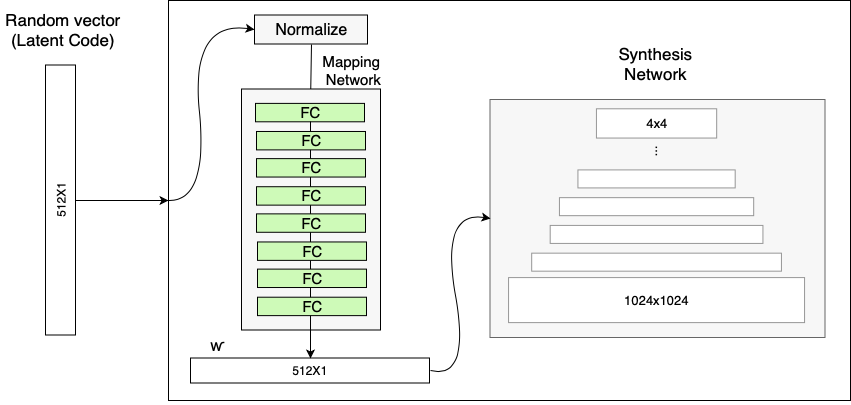
\includegraphics[width=0.8\linewidth]{figures/Mapping-network.png}
	\caption{Mapping Network}
	\label{fig:MappingNetwork}
\end{figure}

Adding this neural network to create an intermediate latent vector would allow the GAN to figure out how it wants to use the numbers in the vector we feed in. Therefore the problem of feature entanglement is alleviated.

\subsection{Adaptive Instance Normalization (AdaIN)}

Suppose we got a latent vector with very low feature entanglement. Maybe the first number of the vector indicates the hair color and the second number determines the gender etc. 

Now think about how do we draw a picture from such description of latent vectors. We do not look at the description once and paint the image immediately. More likely we will first paint the hair, look at another description detail again and then paint another style. 

So, instead of feed the latent vector to the generator once for all, StyleGAN feeds the latent code to every layer of the generator independently.

In order to apply this idea, StyleGAN uses \textbf{Adaptive Instance Normalization}. AdaIN is the learned affine transformation (actually equivalent to linear layer).

\begin{equation}
    y = (y_s, y_b) = f(w)haiyou
\end{equation}

\begin{equation}
    AdaIN(x_i, y)=y_s \frac{x_i - \mu (x)}{\sigma(x)} +y_b
\end{equation}

Here, $x_i$ is the input of every layer in the generator and $y$ comes from the latent vector.

\subsection{Constant Input}

Once again, let us think about drawing a ground true picture by hand. All images from the same kind will have a roughly similar skeleton and we just add and modify several details and styles. But in traditional GAN, the only source of variation and stylistic data is the input latent vector so we have to keep it varying. 

However, in StyleGAN, the style and details can be controlled by mapping network and AdaIN, so it is alright to keep the input of generator a constant tensor to indicate the skeleton of an image. Note that it is the input of generator that is a constant - not the input of mapping network. Thus we have the basic architecture of StyleGAN in Figure \ref{fig:BasicArchitectureofStyleGAN}.

\begin{figure}[h]
	\centering
	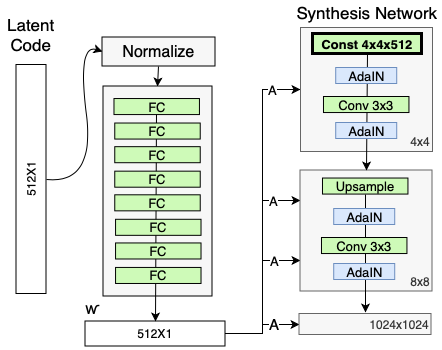
\includegraphics[width=0.7\linewidth]{figures/Constant-input.png}
	\caption{Basic Architecture of StyleGAN}
	\label{fig:BasicArchitectureofStyleGAN}
\end{figure}

\subsection{Style Mixing}

Because the latent vector is injected into every layer independently, so we can inject several different latent vector in different layers in order to get a mixture feature style of them.

In the experiment that NVIDIA makes, 3 different vectors were injected into 3 different spots:

\begin{enumerate}
    \item At the “coarse” layers, where layers where the hidden representation is spatially small — from $4 \times 4$ to $8 \times 8$.
    \item At the “medium” layers, where layers where the hidden representation is medium sized — from $16 \times 16$ to $32 \times 32$.
    \item At the “fine” layers, where layers where the hidden representation is spatially large — from $64 \times 64$ to $1024 \times 1024$.
\end{enumerate}

The spots seems to be set in a not-even way, but it is reasonable because the generator quickly picks up on information and the larger layers mostly refine and sharpen the outputs from the previous layers.

As a result, the mixture output will combine the feature of all three original images (e.g. the mixture faked face may have the same hair color as original image 1 but the same skin color as image 2).

\subsection{Stochastic Noise}

In order to make the generated image more convincing, StyleGAN introduces the \textbf{Stochastic Noise}, which contribute to slightly different hairstyles or freckles. Because we keep the input of generator a constant, so we all apply layer-wise noise injection rather than modifying the latent vector. 

The final architecture of StyleGAN is shown in Figure \ref{fig:FinalArchitectureofStyleGAN}.

\begin{figure}[h]
	\centering
	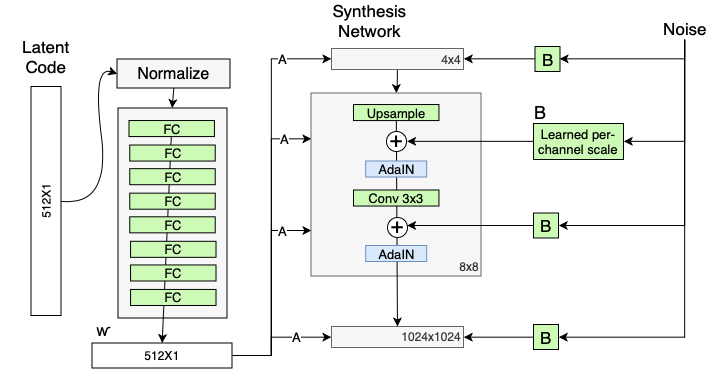
\includegraphics[width=0.85\linewidth]{figures/FinalStyleGAN.png}
	\caption{Final Architecture of StyleGAN}
	\label{fig:FinalArchitectureofStyleGAN}
\end{figure}

\section{Summary of GAN zoos}

This part I summarize the basic idea of some GANs while I go through the papers blogs and documents. Some details may be missing because I do not have time to read them line by line.

\subsection{DCGAN: Deep Convolutional GAN}

DCGAN apply the transposed convolutions to the generator and discriminator network instead of the simple linear layers in the original GAN. It improves the quality of generated images.

\subsection{CGAN: Conditional GAN}

In traditional GAN, we can only generate images from a random noise vector $z$, but can not control the exact kind of the output - we are not sure the output will be a car, a trunk or a train. By adding auxiliary information (e.g. class type, texture description or voices) to \textbf{both the generator and discriminator network}, CGAN can control the output to be what we want it to be.

As for how to combine the auxiliary information, simply concating two tensors is alright. Also, if the information is the class type of the image, use one-hot vector code to encode it.

\subsection{CycleGAN}

CycleGAN provides an unsupervised solution for unpaired image to image translation. CycleGAN operates on two domain $X$ and $Y$, consisting of two generators $G_{X \rightarrow Y}$ and $F_{Y \rightarrow X}$, and two discriminators $D_X$ and $D_Y$. The core idea is \textbf{cycle consistency}:

\begin{equation}
    F(G(x)) \approx x, x \in X
\end{equation}

\begin{equation}
    G(F(y)) \approx y, y \in Y
\end{equation}

Thus we will add a cycle consistency loss to the original loss of generator:

\begin{equation}
    L_{GAN}(G, D_Y, X, Y)=E_y[log(D_Y(y))]+E_x[log(1-D_Y(G(x))]
\end{equation}

\begin{equation}
    L_{cycle}=E_x[||F(G(x))-x||_1]+E_y[||G(F(y))-y||_1]
\end{equation}

\begin{equation}
    Loss = L_{GAN}+L_{cycle}
\end{equation}

\subsection{CoGAN: Coupled GAN}

CoGAN provides an unsupervised solution to learn joint distribution of data from different domains and it consists of two generators and two discriminators. But it have an assumption that domain $X$ and domain $Y$ have highly similar semantic similarity.

Based on this assumption, CoGAN learned joint distribution by enforcing weight sharing constraint on its high level representation weights and then sharpen each domain's detail respectively. Thus the output of $G_1$ and $G_2$ will have some kind of corresponding relations. 

The core idea of CoGAN is shown in Figure \ref{fig:CoGAN}.

\begin{figure}[h]
	\centering
	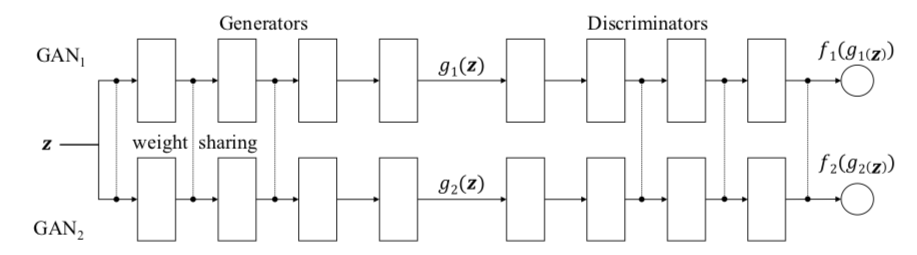
\includegraphics[width=0.85\linewidth]{figures/CoGAN.png}
	\caption{CoGAN}
	\label{fig:CoGAN}
\end{figure}

\subsection{ProGAN: Progressive Growing of GAN}

It is painful to train a GAN model due to the training instability - sometimes the loss of the GAN oscillates or even explode. ProGAN is a technique that helps stabilize GAN training by incrementally increasing the resolution of the generated image.

Instead of directly generate a $1024 \times 1024$ image, we will start from a $4 \times 4$ image and gradually increase the image resolution to $8 \times 8$, $16 \times 16$ and finally $1024 \times 1024$. Also when feed a $1024 \times 1024$ image to the discriminator, we also apply such a degressively process from $1024 \times 1024$ to $512 \times 512$, $256 \times 256$ and finally a scalar.

The architecture of ProGAN is shown in Figure \ref{fig:ProGAN}.

\begin{figure}[h]
	\centering
	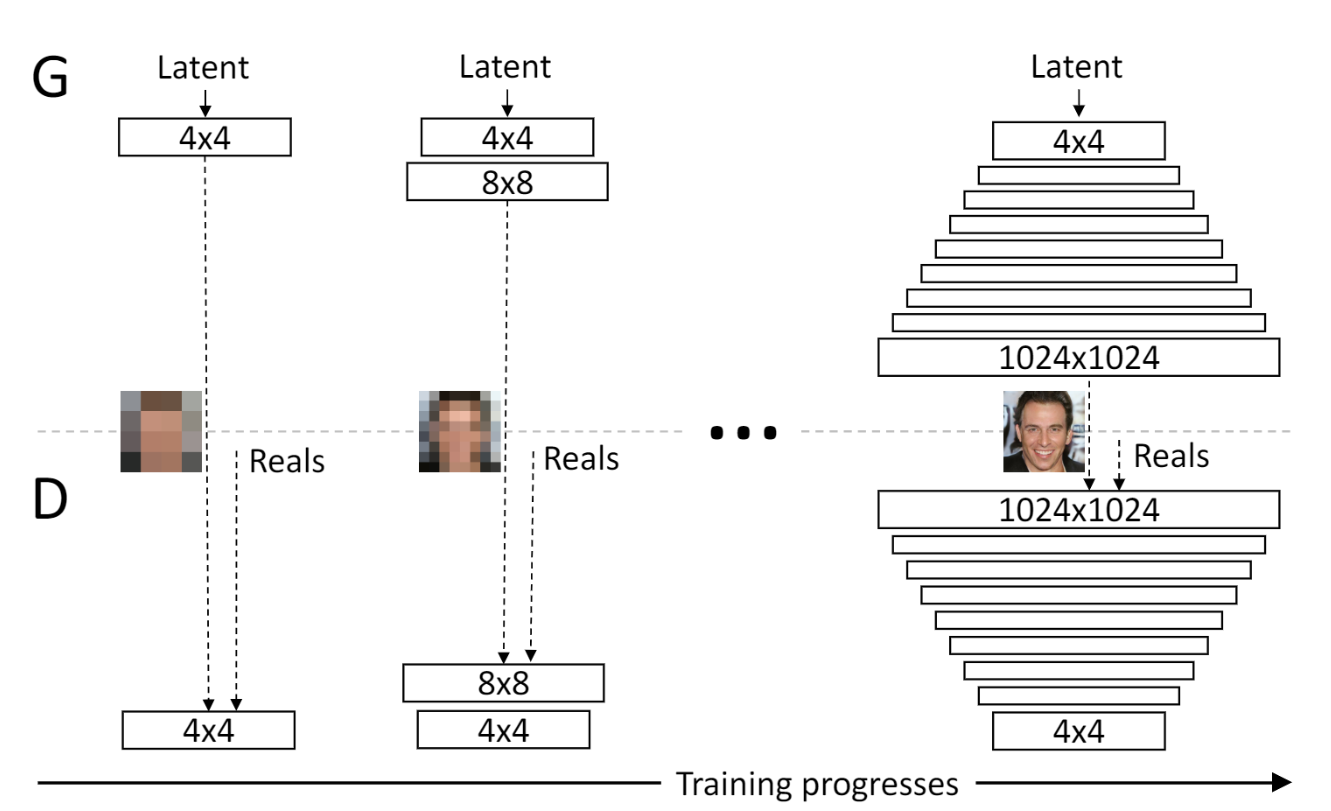
\includegraphics[width=0.75\linewidth]{figures/ProGAN.png}
	\caption{ProGAN}
	\label{fig:ProGAN}
\end{figure}

\subsection{StarGAN}

In area of image to image translation, most models like CycleGAN can only tranform from one domain to another. But what if we want to transform in multiple domains? We should train $k \times (k-1)$ GAN models, which is definitely impracticable. StarGAN comes up with an idea to solve this problem using only one generator.

\begin{figure}[h]
	\centering
	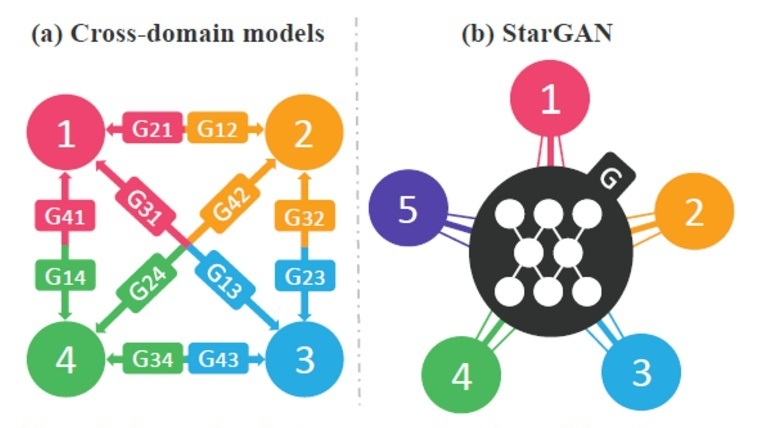
\includegraphics[width=0.75\linewidth]{figures/StarGAN_1.jpg}
	\caption{StarGAN}
	\label{fig:StarGAN_1}
\end{figure}

The generator takes an image and the target domain as inputs and generates the corresponding fake image. The discriminator takes an image as an input and output a scalar indicating whether it is real or not and a domain classification. 

The core of training is similar to cycle consistency. When we re-generate an image from the target domain back to the original domain, the output should be as close as the original input image. The architecture of StarGAN is shown in Figure \ref{fig:StarGAN_2}.

\begin{figure}[h]
	\centering
	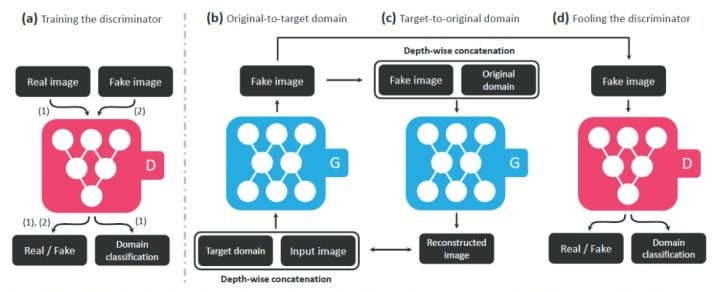
\includegraphics[width=0.95\linewidth]{figures/stargan_2.jpg}
	\caption{Architecture of StarGAN}
	\label{fig:StarGAN_2}
\end{figure}

\section{Implementation and Practice}

\subsection{CGAN on MNIST}

Last time I mentioned that I failed to build a CGAN based on CONV layers. This might be a way too much step for me. So this time I start from the original CGAN, which is built by pure linear neurons and ReLU activations without convolutional or pooling operations.

The CGAN is built and Figure \ref{fig:CGAN_MSELoss} show the generated images from the initial CGAN after 200-epoch training. But it is obviously dissatisfying. After carefully checking the codes and comparing them to the source code on Github, I find out that I mistakenly pick the MSE Loss instead of BCE Loss! I even do not know how I could make this stupid mistake :(

\begin{figure}[h]
	\centering
	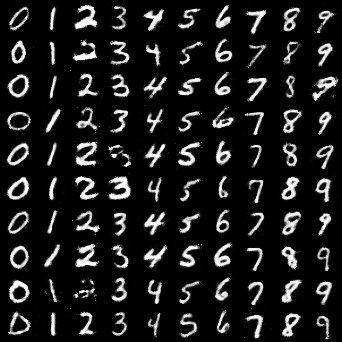
\includegraphics[width=0.4\linewidth]{figures/CGAN_MSELoss.png}
	\caption{Output of initial CGAN}
	\label{fig:CGAN_MSELoss}
\end{figure}

After correcting the loss mistake, I train the model for 800 epochs. As we can see in Figure \ref{fig:CGAN_BCELoss}, the quality of generated images continue growing as the training process moves on. And after 800-epoch training, I think the generated images are rather realistic despite a little pixel blurry.

\begin{figure}[htbp]
\centering
\subfigure[Epoch 200]{
\begin{minipage}[t]{0.35\linewidth}
\centering
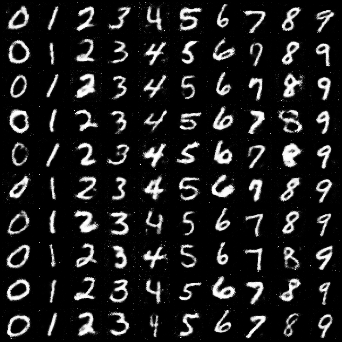
\includegraphics[width=1.7in]{figures/CGAN_BCELoss200.png}
%\caption{fig2}
\end{minipage}%
}%
\subfigure[Epoch 400]{
\begin{minipage}[t]{0.35\linewidth}
\centering
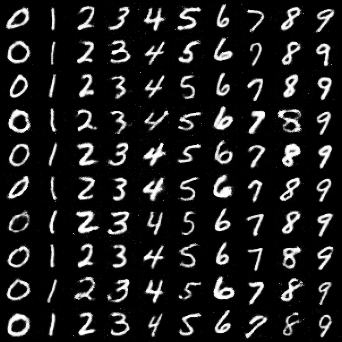
\includegraphics[width=1.7in]{figures/CGAN_BCELoss400.png}
%\caption{fig2}
\end{minipage}
}%
\centering
\end{figure}

\begin{figure}[htbp]
\centering
\subfigure[Epoch 600]{
\begin{minipage}[t]{0.35\linewidth}
\centering
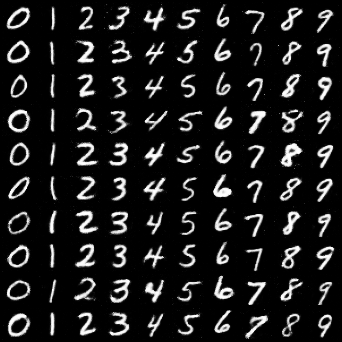
\includegraphics[width=1.7in]{figures/CGAN_BCELoss600.png}
%\caption{fig2}
\end{minipage}%
}%
\subfigure[Epoch 800]{
\begin{minipage}[t]{0.35\linewidth}
\centering
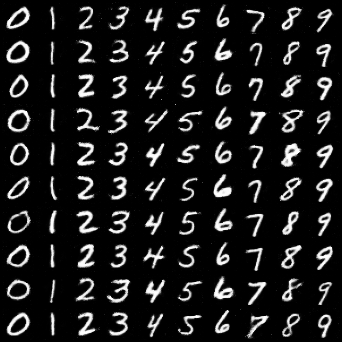
\includegraphics[width=1.7in]{figures/CGAN_BCELoss800.png}
%\caption{fig2}
\end{minipage}
}%
\centering
\caption{Output of corrected CGAN}
\label{fig:CGAN_BCELoss}
\end{figure}

Additionally, as we all known, the latent vector $z$ somehow represents the feature of the generated images. So I think maybe dimension $100$ is so large for simple images in MNIST dataset (only hand write numbers from $0$ to $9$) that it can cause code information redundancy and feature entanglement. Therefore, I try to reduce the dimension of latent vector from $100$ to $10$, but it turn out a bad result shown in Figure \ref{fig:CGAN_latent_dim_10}. 

\begin{figure}[h]
	\centering
	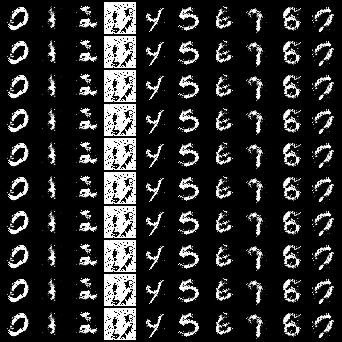
\includegraphics[width=0.4\linewidth]{figures/CGAN_latent_dim_10.png}
	\caption{CGAN with latent dimension of 10}
	\label{fig:CGAN_latent_dim_10}
\end{figure}

In my opinion, it is because the latent space are too small to extract the full information for image generation. This means that a seemingly simple image (e.g. hand-write number $0$) can contain many feature information for machines which humans may not notice.

\subsection{DCGAN on MNIST}

Last time I built a DCGAN model, trained it for 50 epochs and considered it converged. But this time I extend the training epoch to 200 and find out that the work I done last time is far away from accomplishment.

As the two figures shown in Figure \ref{fig:DCGANoutput}, after 50-epoch training last time, the generated images still greatly suffer from blurry strokes with white pixel points scattering around, which can be easily judged to be fake one by a human being. However, after 200-epoch training this time, the generated strokes are so clean, clear and sharply that one can not easily say it is faked or not in spite of the semantic interpretation of some weird images.

\begin{figure}[htbp]
\centering
\subfigure[Output of generator last time]{
\begin{minipage}[t]{0.5\linewidth}
\centering
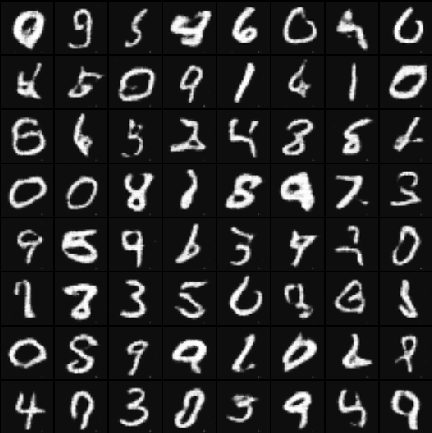
\includegraphics[width=2.5in]{figures/DCGAN_lasttime.png}
%\caption{fig2}
\end{minipage}%
}%
\subfigure[Output of generator this time]{
\begin{minipage}[t]{0.5\linewidth}
\centering
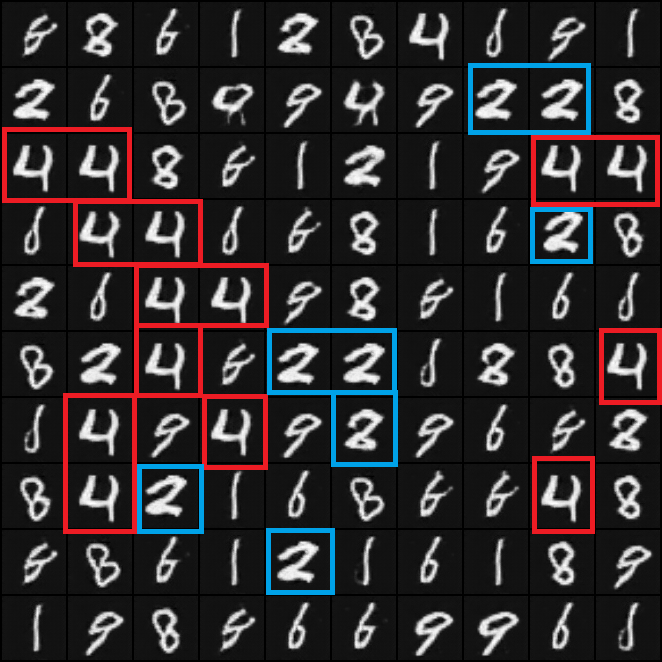
\includegraphics[width=2.5in]{figures/DCGAN_thistime.png}
%\caption{fig2}
\end{minipage}
}%
\centering
\caption{Output of Generator Network}
\label{fig:DCGANoutput}
\end{figure}

We can see that most of the generated images clearly indicate a corresponding number. Nevertheless, some of them are just uninterpretable strange symbols. I think this is due to the basic idea of GAN. The goal of GAN is to make the distribution $p_G$ exactly the same as $p_{data}$, but two distribution must have overlaps and differences. The generator may combine the strokes of different numbers and thus create a weird symbol. Therefore, next time I will try to combine the DCGAN with CGAN, which should solve both the problems - semantic interpretation and clearly strokes.

Also, I notice that many generated images are exactly the same (I have labeled some of them using red and blue box selections), which means that mode collapse has \textbf{partially} taken place. Actually this bad smell occurs when I print out the intermediate output graphs (shown in Figure \ref{fig:DCGANIntermediate}). Unfortunately, I have not come up with ideas to successfully solve it up to now :(

\begin{figure}[htbp]
\centering
\subfigure[Epoch 19]{
\begin{minipage}[t]{0.3\linewidth}
\centering
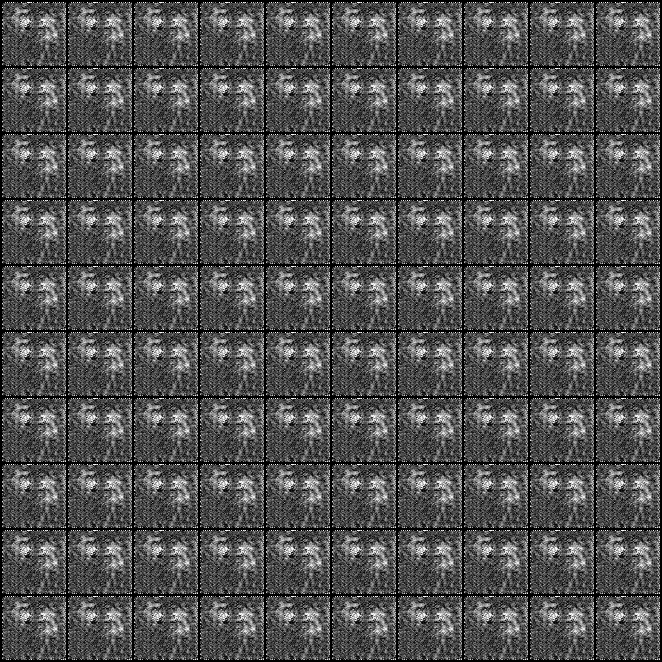
\includegraphics[width=1.5in]{figures/DCGAN19.png}
%\caption{fig2}
\end{minipage}%
}%
\subfigure[Epoch 21]{
\begin{minipage}[t]{0.3\linewidth}
\centering
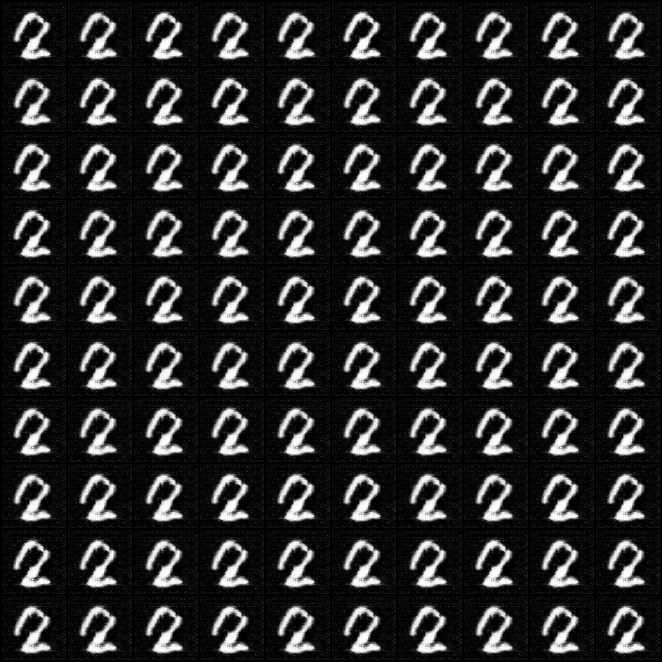
\includegraphics[width=1.5in]{figures/DCGAN21.png}
%\caption{fig2}
\end{minipage}
}%
\centering
\end{figure}

\begin{figure}[htbp]
\centering
\subfigure[Epoch 23]{
\begin{minipage}[t]{0.3\linewidth}
\centering
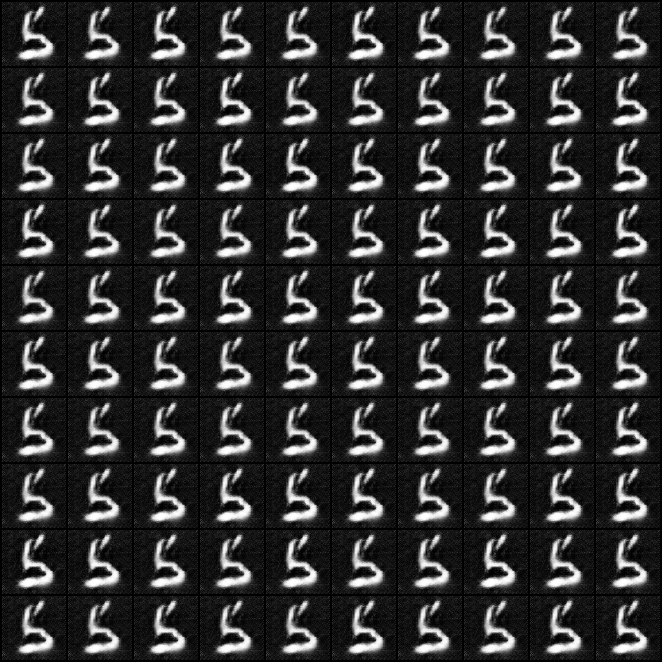
\includegraphics[width=1.5in]{figures/DCGAN23.png}
%\caption{fig2}
\end{minipage}%
}%
\subfigure[Epoch 25]{
\begin{minipage}[t]{0.3\linewidth}
\centering
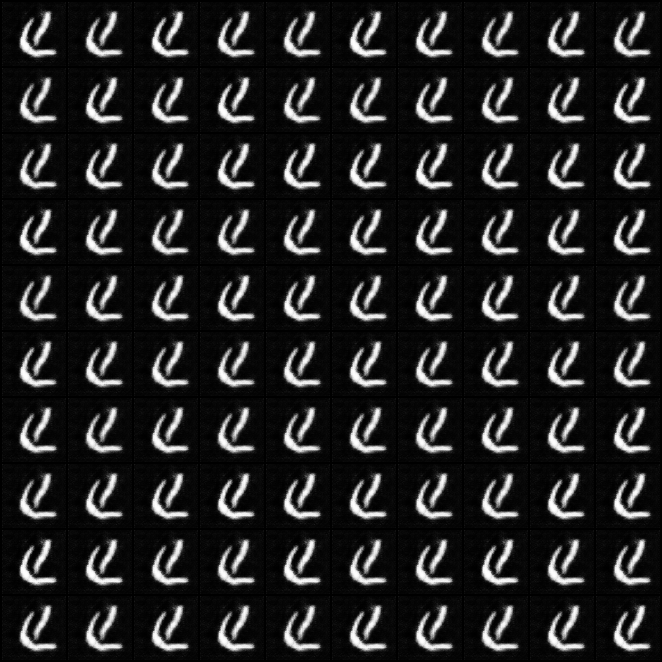
\includegraphics[width=1.5in]{figures/DCGAN25.png}
%\caption{fig2}
\end{minipage}
}%
\centering
\caption{Intermediate Images of DCGAN}
\label{fig:DCGANIntermediate}
\end{figure}

\section{Work Next Week}

\begin{itemize}
    \item Paper about BigBiGAN
    \item Presentation about StyleGAN
    \item Try to implement more complex GAN model
    \item Fill in the summary of GAN zoo
\end{itemize}

\end{document}